% =======================================================================================
\section{Fisher Forecast}
\label{app:fisher}
% =======================================================================================
% added 2026-11-19 (user): every Fisher part in one appendix, moved from app:evaluation and app:mcmc; trimmed the same
% day to a cross-check (user: "just a double check when useful"). Dropped: the q-space draw formula, the Hessian
% statistics of the old prior (fisher-diagonal.json, log Mc; their TODO(new runs) with them), the full-band fdot
% overflow TODO (now one clause), the ideal-width figure (figures/fisher-width.pdf).

Every eval source also gets a Fisher forecast, a cheap Gaussian width used as a cross-check; the results
are read against the joint chains (\cref{app:mcmc,app:results}).

\subsection{The Forecast}
\label{app:evaluation-fisher}\label{app:fisher-forecast}

Each eval injection gets a Gaussian centred at the truth $\theta^\star$ with precision
\begin{equation}
  \Gamma = \frac1{N_{\rm F}}\sum_{r=1}^{N_{\rm F}}\nabla^2_\theta\bigl[-\log L(\theta; d_r)\bigr]_{\theta^\star}
  + \Lambda,
  \qquad N_{\rm F} = \EvaluationFisherDraws,
  \label{eq:evaluation-fisher}
\end{equation}
the Hessian of \cref{eq:loglik} averaged over noise realisations $d_r$, which is the Fisher matrix
\citep{cutler1994gravitational,vallisneri2008use}, plus $\Lambda$, a Gaussian stand-in for the prior that keeps
poorly measured directions at the prior's width. It is drawn with $\log\fdot$ in place of $\fdot$, and each
eigenvalue is floored at the prior's precision along its eigenvector. Being unimodal and Gaussian, it misses
the exact symmetries of \cref{eq:psi-phi-symmetry} and the curved amplitude--inclination degeneracy, and where
the data barely constrain a parameter it returns the prior's width: $\fdot$ for most of the narrow band, and
the faint sources of the full band, whose $\log\fdot$ draws it does not bound (we do not use them).

\subsection{Against the Ideal Width and the Joint \acs{mcmc}}
\label{app:mcmc-fisher}\label{app:fisher-ideal}

The forecast's $f_0$ width is never below the ideal width of \cref{eq:evaluation-ideal-width}: a median
\EvaluationFisherRatioNarrow{} times it in the narrow band, where the chirp is barely measured, and
\EvaluationFisherRatioFull{} in the full band, where a measured chirp costs up to the factor
\EvaluationStartFactor{} of a start-of-observation $f_0$. On the full band the Fisher width is therefore the
sharper yardstick.

\begin{figure}[!htbp]
  \centering
  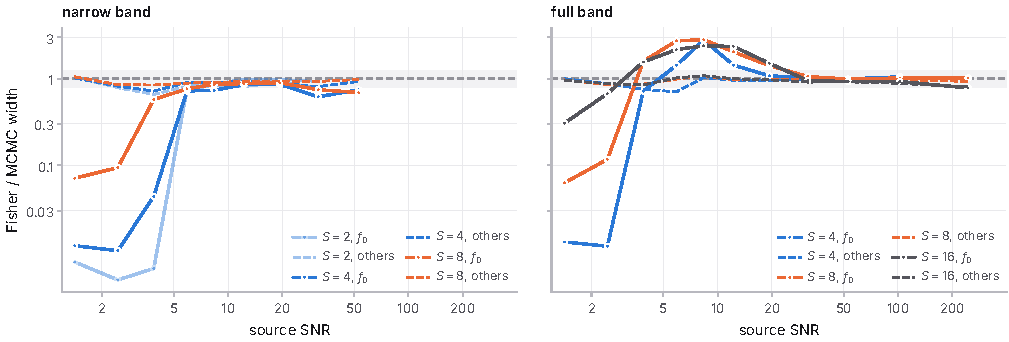
\includegraphics{figures/mcmc.pdf}
  \caption{Fisher widths over the joint \ac{mcmc} widths of the six references, per band (panels) and
  source count (colours): the median over the sources in each \ac{snr} bin of the $f_0$ ratio (solid) and of
  the median ratio of the six parameters other than $f_0$ and $\fdot$ (dashed); the shaded band is
  \McmcFisherLo--\McmcFisherHi. From \ac{snr} \McmcFisherMidSnr{} up the forecast sits in the band.}
  \label{fig:mcmc-widths}
\end{figure}

Against the chains (\cref{fig:mcmc-widths}), from \ac{snr} \McmcFisherHighSnr{} up the forecast's median width
per parameter is \McmcFisherHighMedianLo--\McmcFisherHighMedianHi{} times theirs, and from \ac{snr}
\McmcFisherMidSnr{} up it is a fair proxy. Below \ac{snr} \McmcFisherFaintSnr{} it is no proxy: the chains
spread a faint source's $f_0$ over much of the window, as the prior does, and the forecast does not. Between
\ac{snr} \McmcFisherFaintSnr{} and \McmcFisherMidSnr{} on the full band it is \McmcFisherFullMidLo--\McmcFisherFullMidHi{}
times wider in $f_0$, partly because the reference is too narrow there (\cref{app:results-mcmc}).
